\documentclass[tikz,border=12pt]{standalone}
\usepackage[T1]{fontenc}
\usepackage{mathpazo}
\usepackage{amsmath,amssymb}
\usetikzlibrary{arrows.meta, positioning, calc}

\definecolor{stblue}{HTML}{7B97AD}
\definecolor{rwgold}{HTML}{B8995E}
\definecolor{sage}{HTML}{7A9A7E}
\definecolor{dkbrown}{HTML}{3D3530}
\definecolor{wmgray}{HTML}{7B7067}
\definecolor{cream}{HTML}{F9F6F0}
\definecolor{border}{HTML}{D4C9B8}
\definecolor{terracotta}{HTML}{C47A6A}
\definecolor{lavender}{HTML}{907EA0}

\begin{document}
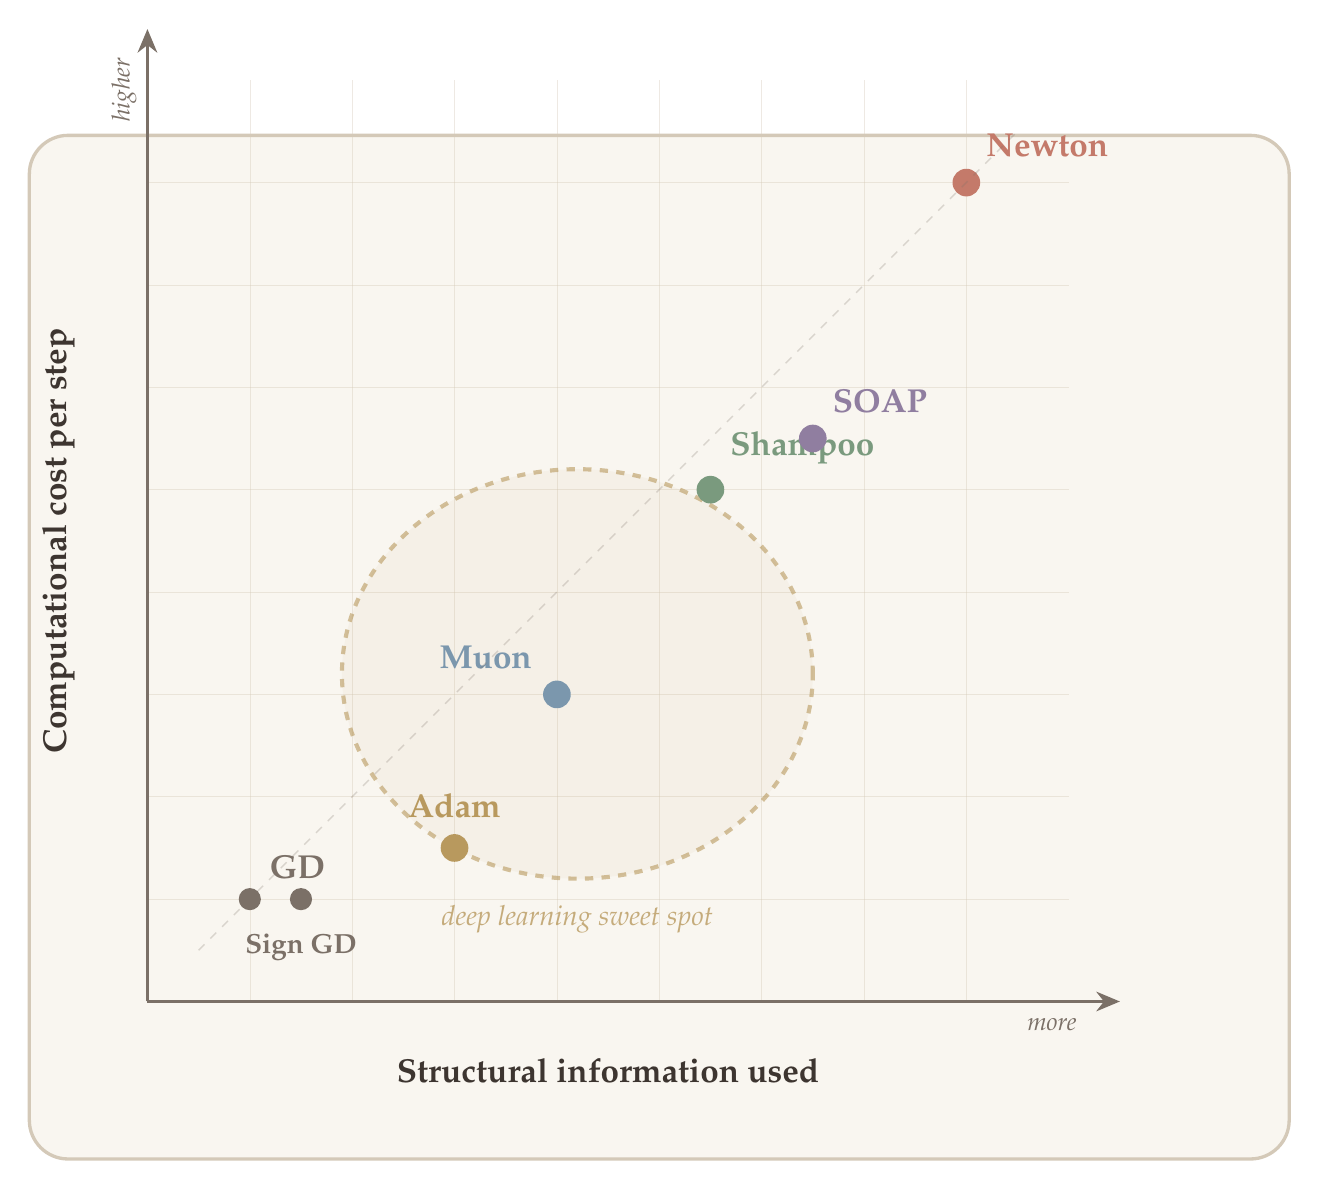
\begin{tikzpicture}[>={Stealth[length=3mm, width=2.5mm]}]

% Background
\fill[cream, rounded corners=14pt] (-1.5,-2.0) rectangle (14.5,11.0);
\draw[border, line width=1.2pt, rounded corners=14pt] (-1.5,-2.0) rectangle (14.5,11.0);

% Axes (scale: 1.3 cm per unit)
\def\s{1.3}

% Light grid
\foreach \v in {1,2,...,8} {
  \draw[border, line width=0.2pt, opacity=0.4] ({\v*\s},0) -- ({\v*\s},{9*\s});
  \draw[border, line width=0.2pt, opacity=0.4] (0,{\v*\s}) -- ({9*\s},{\v*\s});
}

% Axis lines
\draw[wmgray, line width=1pt, ->] (0,0) -- ({9.5*\s},0);
\draw[wmgray, line width=1pt, ->] (0,0) -- (0,{9.5*\s});

% Axis labels
\node[text=dkbrown, font=\large\bfseries, anchor=north] at ({4.5*\s},-0.6) {Structural information used};
\node[text=dkbrown, font=\large\bfseries, rotate=90, anchor=south] at (-0.8,{4.5*\s}) {Computational cost per step};

% Arrows on axes
\node[text=wmgray, font=\small\itshape, anchor=west] at ({8.5*\s},-0.3) {more};
\node[text=wmgray, font=\small\itshape, rotate=90, anchor=west] at (-0.3,{8.5*\s}) {higher};

% Deep learning sweet spot ellipse
\draw[rwgold, dashed, line width=1.5pt, opacity=0.6]
  ({4.2*\s},{3.2*\s}) ellipse ({2.3*\s} and {2.0*\s});
\fill[rwgold, opacity=0.06]
  ({4.2*\s},{3.2*\s}) ellipse ({2.3*\s} and {2.0*\s});
\node[text=rwgold, font=\normalsize\itshape, opacity=0.8] at ({4.2*\s},{0.8*\s}) {deep learning sweet spot};

% Points with labels
% GD (1, 1)
\fill[wmgray] ({1*\s},{1*\s}) circle (4pt);
\node[text=wmgray, font=\large\bfseries, anchor=south west] at ({1.1*\s},{1.1*\s}) {GD};

% Sign GD (1.5, 1)
\fill[wmgray] ({1.5*\s},{1*\s}) circle (4pt);
\node[text=wmgray, font=\normalsize\bfseries, anchor=north] at ({1.5*\s},{0.75*\s}) {Sign GD};

% Adam/AdamW (3, 1.5)
\fill[rwgold] ({3*\s},{1.5*\s}) circle (5pt);
\node[text=rwgold, font=\large\bfseries, anchor=south] at ({3*\s},{1.7*\s}) {Adam};

% Muon (4, 3)
\fill[stblue] ({4*\s},{3*\s}) circle (5pt);
\node[text=stblue, font=\large\bfseries, anchor=south east] at ({3.85*\s},{3.15*\s}) {Muon};

% Shampoo (5.5, 5)
\fill[sage] ({5.5*\s},{5*\s}) circle (5pt);
\node[text=sage, font=\large\bfseries, anchor=south west] at ({5.6*\s},{5.15*\s}) {Shampoo};

% SOAP (6.5, 5.5)
\fill[lavender] ({6.5*\s},{5.5*\s}) circle (5pt);
\node[text=lavender, font=\large\bfseries, anchor=south west] at ({6.6*\s},{5.65*\s}) {SOAP};

% Newton (8, 8)
\fill[terracotta] ({8*\s},{8*\s}) circle (5pt);
\node[text=terracotta, font=\large\bfseries, anchor=south west] at ({8.1*\s},{8.15*\s}) {Newton};

% Faint diagonal
\draw[wmgray, line width=0.5pt, opacity=0.25, dashed] ({0.5*\s},{0.5*\s}) -- ({8.5*\s},{8.5*\s});

\end{tikzpicture}
\end{document}
